%
% STAT 100: Chance and Data Analysis - A Course Overview
% Section: Analysis of Multi-Variable Data
%
% Author: Jeffrey Leung
%

\section{Analysis of Multi-Variable Data}
	\label{sec:analysis-of-multi-variable-data}
\subsection{Relationships between Two Quantitative Variables}
	\label{subsec:analysis-of-multi-variable-data:relationships-between-two-quantitative-variables}
\begin{easylist}

	& Relationships between two quantitative variables:
	& \emph{Dependent/respondent variable:} Variable to be predicted
		&& Placed on the vertical (y) axis
	& \emph{Independent variable/predictor:} Variable used to predict the dependent variable
		&& Placed on the horizontal (x) axis
	& \emph{Scatterplot:} Visual comparisons of the values of two quantitative variables (see figure %TODO in bullet point?
	
	& \emph{positive/negative:}
	
	& Forms and strength of a relationship:
		&& \emph{Linear:} Approximate change in values can be summarized in a single 2-d direction
			&&& I.e. Points which follow a straight line
		&& \emph{Non-linear:} Values change in multiple 2-d directions
			&&& E.g. Exponential functions, trigonometric functions
			
		&& \emph{Strength:} Denseness of distribution which shows a clear form/relation
			&& 
		
	& \emph{Correlation coefficient:} Value which denotes the strength of the data
			&&& Denoted by $r$
			&&& Formula: $r = $
			&&& Value:
				&&&& $-1 \leq r \leq 1$
				&&&& Closer to -1, the data is more negatively related
				&&&& Closer to 0, the data is more weakly related 
				&&&& Closer to 1, the data is more positively related
			&&& Interpretation: The closer to 1 $r$ is, the stronger the correlation
			&&& Only applies to linear data
				&&&& 0 for non-linear data
			&&& Outliers may need to be removed before calculation
			&&& E.g. The correlation coefficient of a midterm grade and a final grade was found to be 0.8747. The relationship between the two grades is positive, strong, and linear.
			
		&& For an interpretation of the magnitude, see table~\ref{tab:strength-of-a-correlation-coefficient}
		
		\Deactivate
		\begin{table}[!htb]
			\centering
			\caption{Strength of a Correlation Coefficient}
			\label{tab:strength-of-a-correlation-coefficient}
			\begin{tabular}{ c l }
				Magnitude of the Correlation Coefficient & Strength \\
				\hline
				$0 < |r| < 0.4$ & Weak \\
				$0.4 \leq |r| < 0.6$ & Moderately weak \\
				$0.6 \leq |r| < 0.8$ & Moderately strong \\
				$0.8 \leq |r| < 1.0$ & Strong \\
				$|r| = 1$ & Perfect
			\end{tabular}
		\end{table}
		\Activate
		
		%TODO incomplete
				
			
	& Correlation:
		&& Declares an association between two variables
		&& Does not imply causation - i.e. an existing linear relationship does not mean a change in the independent variable causes a change in the dependent variable (see figure~\ref{fig:xkcd-552})
	
	\begin{figure}[!htb]
		\centering
		\caption{XKCD Webcomic - 552: Correlation}
		\label{fig:xkcd-552}
		\href{https://xkcd.com/552/}{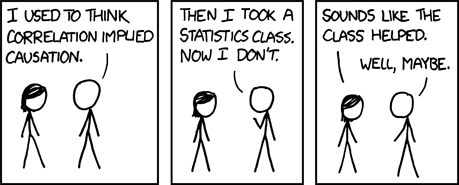
\includegraphics[scale=.75]{xkcd-552-correlation}}
	\end{figure}
		
		
	& \emph{Lurking variable:} Variable outside of the tested variables which explains an association between the two tested variables
		
	& \emph{Regression analysis:}
		&& \emph{Regression line:} Best-fit line
			&&& Before using the regression line to predict data, check data ranges
		&& %TODO
		&& \emph{Regression equation:} Mathematical equation of a regression line
			&&& May have multiple $x$ variables
			&&& Formula: $y = slope_1 \cdot x_1 + slope_2 \cdot x_2 + \ldots + slope_n \cdot x_n + y_{intercept}$
				&&&& Where $y =$ dependent variable, and $x_1, x_2, \ldots, x_n =$ independent variables
				&&&& Use a scientific calculator to determine the intercept and slope %TODO how
			&&& Cannot be used to predict data less than the minimum or greater than the maximum because there is no data to support the analysis
			&&& Slope of a regression equation: $\frac{y_{2} - y_{1}}{x_{2} - x_{1}}$
				&&&& Per 1 unit change in $x$, $y$ should change by the value of the slope
				&&&& Example of interp: For every 1 additional $x$, we predict $y$ will change by $slope$.
		&& \emph{Coefficient of determination:}
			&& Denoted by $R^{2}$
			&& Value:
				&&& $R^{2} = r^2$ where $r =$ the correltion coefficient
				&& $0 \leq R^{2} \leq 1$
			&& Interpretation: $R^{2}$ represents the variability in percent which can be explained by the regression line.
			%TODO notes
		
	& Multiple regression:
		&& See video
		&& Use excel
		
	
		
\end{easylist}
\clearpage